\documentclass{standalone}
\usepackage{tikz}
\usetikzlibrary{patterns, positioning}
\usepackage[sfdefault]{ClearSans} %% option 'sfdefault' activates Clear Sans as the default text font
\usepackage[T1]{fontenc}

\begin{document}
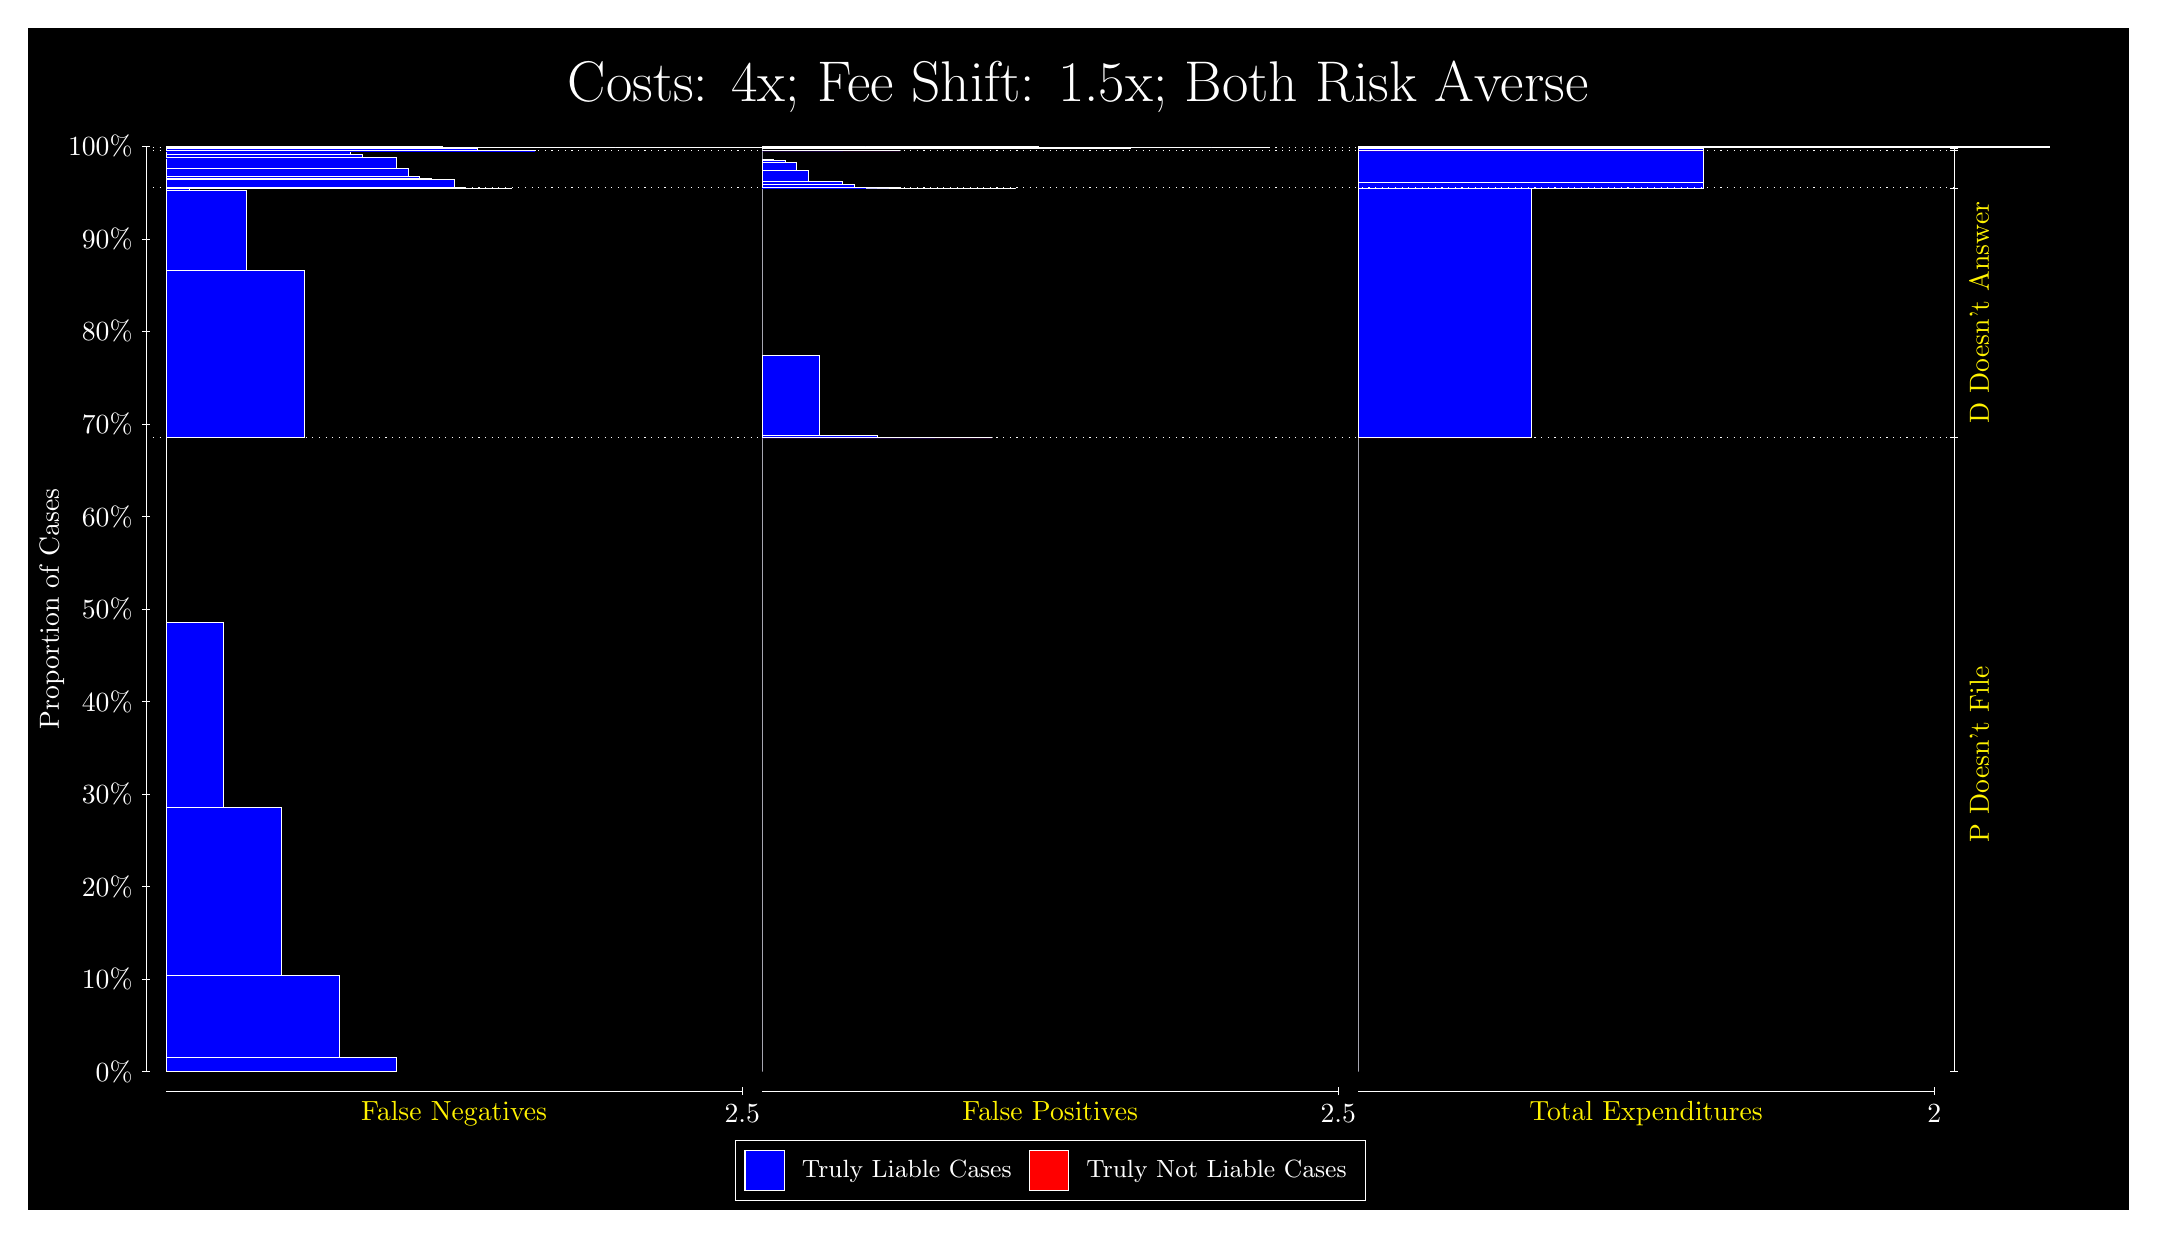
\begin{tikzpicture}
\draw[fill=black] (0,0) rectangle (26.667,15);
\draw[text=white] (0,13.5) rectangle (26.667,15) node[midway] {\huge Costs: 4x; Fee Shift: 1.5x; Both Risk Averse};
\draw[white, very thin] (1.5,1.75) -- (1.5,13.5);
\node[rotate=90, text=white, anchor=center] at (0.3, 7.625) {Proportion of Cases};
\draw[white, very thin] (1.45,1.75) -- (1.55,1.75);
\node[text=white, anchor=east] at (1.45, 1.75) {0\%};
\draw[white, very thin] (1.45,2.925) -- (1.55,2.925);
\node[text=white, anchor=east] at (1.45, 2.925) {10\%};
\draw[white, very thin] (1.45,4.1) -- (1.55,4.1);
\node[text=white, anchor=east] at (1.45, 4.1) {20\%};
\draw[white, very thin] (1.45,5.275) -- (1.55,5.275);
\node[text=white, anchor=east] at (1.45, 5.275) {30\%};
\draw[white, very thin] (1.45,6.45) -- (1.55,6.45);
\node[text=white, anchor=east] at (1.45, 6.45) {40\%};
\draw[white, very thin] (1.45,7.625) -- (1.55,7.625);
\node[text=white, anchor=east] at (1.45, 7.625) {50\%};
\draw[white, very thin] (1.45,8.8) -- (1.55,8.8);
\node[text=white, anchor=east] at (1.45, 8.8) {60\%};
\draw[white, very thin] (1.45,9.975) -- (1.55,9.975);
\node[text=white, anchor=east] at (1.45, 9.975) {70\%};
\draw[white, very thin] (1.45,11.15) -- (1.55,11.15);
\node[text=white, anchor=east] at (1.45, 11.15) {80\%};
\draw[white, very thin] (1.45,12.325) -- (1.55,12.325);
\node[text=white, anchor=east] at (1.45, 12.325) {90\%};
\draw[white, very thin] (1.45,13.5) -- (1.55,13.5);
\node[text=white, anchor=east] at (1.45, 13.5) {100\%};

\draw[white, very thin] (24.457,1.75) -- (24.457,13.5);
\draw[white, very thin] (24.407,1.75) -- (24.507,1.75);
\node[anchor=west] at (24.407, 1.75) {};
\draw[white, very thin] (24.407,9.8005) -- (24.507,9.8005);
\node[anchor=west] at (24.407, 9.8005) {};
\draw[white, very thin] (24.407,12.973) -- (24.507,12.973);
\node[anchor=west] at (24.407, 12.973) {};
\draw[white, very thin] (24.407,13.444) -- (24.507,13.444);
\node[anchor=west] at (24.407, 13.444) {};
\draw[white, very thin] (24.407,13.48) -- (24.507,13.48);
\node[anchor=west] at (24.407, 13.48) {};
\draw[white, very thin] (24.407,13.488) -- (24.507,13.488);
\node[anchor=west] at (24.407, 13.488) {};
\draw[white, very thin] (24.407,13.5) -- (24.507,13.5);
\node[anchor=west] at (24.407, 13.5) {};

\draw[white, very thin, fill=blue] (1.75,1.75) rectangle (4.6775,1.9353);
\draw[white, very thin, fill=blue] (1.75,1.9353) rectangle (3.9457,2.9724);
\draw[white, very thin, fill=blue] (1.75,2.9724) rectangle (3.2138,5.1023);
\draw[white, very thin, fill=blue] (1.75,5.1023) rectangle (2.4819,7.4505);
\draw[white, very thin, fill=red] (1.75,7.4505) rectangle (1.75,7.4505);
\draw[white, very thin, fill=blue] (1.75,7.4505) rectangle (1.75,9.8005);
\draw[white, very thin, fill=blue] (1.75,9.8005) rectangle (3.5065,11.923);
\draw[white, very thin, fill=blue] (1.75,11.923) rectangle (2.7746,12.941);
\draw[white, very thin, fill=blue] (1.75,12.941) rectangle (2.0428,12.973);
\draw[white, very thin, fill=red] (1.75,12.973) rectangle (1.75,12.973);
\draw[white, very thin, fill=blue] (1.75,12.973) rectangle (1.75,12.973);
\draw[white, very thin, fill=blue] (1.75,12.973) rectangle (6.1413,12.973);
\draw[white, very thin, fill=blue] (1.75,12.973) rectangle (5.8486,12.973);
\draw[white, very thin, fill=blue] (1.75,12.973) rectangle (5.5558,12.978);
\draw[white, very thin, fill=blue] (1.75,12.978) rectangle (5.4094,13.082);
\draw[white, very thin, fill=blue] (1.75,13.082) rectangle (5.2631,13.085);
\draw[white, very thin, fill=blue] (1.75,13.085) rectangle (5.1167,13.09);
\draw[white, very thin, fill=blue] (1.75,13.09) rectangle (4.9703,13.123);
\draw[white, very thin, fill=blue] (1.75,13.123) rectangle (4.8239,13.218);
\draw[white, very thin, fill=blue] (1.75,13.218) rectangle (4.6775,13.355);
\draw[white, very thin, fill=blue] (1.75,13.355) rectangle (4.5312,13.358);
\draw[white, very thin, fill=blue] (1.75,13.358) rectangle (4.3848,13.364);
\draw[white, very thin, fill=blue] (1.75,13.364) rectangle (4.2384,13.402);
\draw[white, very thin, fill=blue] (1.75,13.402) rectangle (4.092,13.44);
\draw[white, very thin, fill=blue] (1.75,13.44) rectangle (3.9457,13.442);
\draw[white, very thin, fill=blue] (1.75,13.442) rectangle (3.7993,13.442);
\draw[white, very thin, fill=blue] (1.75,13.442) rectangle (3.6529,13.442);
\draw[white, very thin, fill=blue] (1.75,13.442) rectangle (3.5065,13.444);
\draw[white, very thin, fill=blue] (1.75,13.444) rectangle (3.3602,13.444);
\draw[white, very thin, fill=blue] (1.75,13.444) rectangle (3.2138,13.444);
\draw[white, very thin, fill=blue] (1.75,13.444) rectangle (3.0674,13.444);
\draw[white, very thin, fill=blue] (1.75,13.444) rectangle (2.921,13.444);
\draw[white, very thin, fill=blue] (1.75,13.444) rectangle (2.7746,13.444);
\draw[white, very thin, fill=blue] (1.75,13.444) rectangle (2.6283,13.444);
\draw[white, very thin, fill=blue] (1.75,13.444) rectangle (2.3355,13.444);
\draw[white, very thin, fill=blue] (1.75,13.444) rectangle (2.0428,13.444);
\draw[white, very thin, fill=red] (1.75,13.444) rectangle (1.75,13.444);
\draw[white, very thin, fill=blue] (1.75,13.444) rectangle (6.4341,13.445);
\draw[white, very thin, fill=blue] (1.75,13.445) rectangle (5.7022,13.475);
\draw[white, very thin, fill=blue] (1.75,13.475) rectangle (4.9703,13.48);
\draw[white, very thin, fill=blue] (1.75,13.48) rectangle (4.2384,13.48);
\draw[white, very thin, fill=blue] (1.75,13.48) rectangle (3.5065,13.48);
\draw[white, very thin, fill=red] (1.75,13.48) rectangle (1.75,13.48);
\draw[white, very thin, fill=blue] (1.75,13.48) rectangle (3.5065,13.48);
\draw[white, very thin, fill=blue] (1.75,13.48) rectangle (2.7746,13.488);
\draw[white, very thin, fill=blue] (1.75,13.488) rectangle (2.0428,13.488);
\draw[white, very thin, fill=red] (1.75,13.488) rectangle (1.75,13.488);
\draw[white, very thin, fill=blue] (1.75,13.488) rectangle (1.75,13.488);
\draw[white, very thin, fill=blue] (1.75,13.488) rectangle (13.46,13.488);
\draw[white, very thin, fill=blue] (1.75,13.488) rectangle (12.728,13.488);
\draw[white, very thin, fill=blue] (1.75,13.488) rectangle (11.996,13.488);
\draw[white, very thin, fill=blue] (1.75,13.488) rectangle (11.265,13.488);
\draw[white, very thin, fill=blue] (1.75,13.488) rectangle (10.533,13.488);
\draw[white, very thin, fill=blue] (1.75,13.488) rectangle (9.8008,13.488);
\draw[white, very thin, fill=blue] (1.75,13.488) rectangle (7.4587,13.488);
\draw[white, very thin, fill=blue] (1.75,13.488) rectangle (6.7268,13.489);
\draw[white, very thin, fill=blue] (1.75,13.489) rectangle (5.9949,13.491);
\draw[white, very thin, fill=blue] (1.75,13.491) rectangle (5.2631,13.497);
\draw[white, very thin, fill=blue] (1.75,13.497) rectangle (4.5312,13.5);
\draw[white, very thin, fill=blue] (1.75,13.5) rectangle (3.7993,13.5);
\draw[white, very thin, fill=blue] (1.75,13.5) rectangle (3.0674,13.5);
\draw[white, very thin, fill=blue] (1.75,13.5) rectangle (2.3355,13.5);
\draw[white, very thin, fill=red] (1.75,13.5) rectangle (1.75,13.5);
\draw[white, very thin, fill=red] (9.3189,1.75) rectangle (9.3189,1.75);
\draw[white, very thin, fill=blue] (9.3189,1.75) rectangle (9.3189,9.8005);
\draw[white, very thin, fill=red] (9.3189,9.8005) rectangle (12.246,9.8005);
\draw[white, very thin, fill=blue] (9.3189,9.8005) rectangle (12.246,9.8005);
\draw[white, very thin, fill=blue] (9.3189,9.8005) rectangle (11.515,9.8005);
\draw[white, very thin, fill=blue] (9.3189,9.8005) rectangle (10.783,9.8321);
\draw[white, very thin, fill=blue] (9.3189,9.8321) rectangle (10.051,10.85);
\draw[white, very thin, fill=blue] (9.3189,10.85) rectangle (9.3189,12.973);
\draw[white, very thin, fill=red] (9.3189,12.973) rectangle (12.539,12.973);
\draw[white, very thin, fill=blue] (9.3189,12.973) rectangle (12.539,12.973);
\draw[white, very thin, fill=red] (9.3189,12.973) rectangle (12.246,12.973);
\draw[white, very thin, fill=blue] (9.3189,12.973) rectangle (12.246,12.973);
\draw[white, very thin, fill=red] (9.3189,12.973) rectangle (11.954,12.973);
\draw[white, very thin, fill=blue] (9.3189,12.973) rectangle (11.954,12.973);
\draw[white, very thin, fill=blue] (9.3189,12.973) rectangle (11.807,12.973);
\draw[white, very thin, fill=red] (9.3189,12.973) rectangle (11.661,12.973);
\draw[white, very thin, fill=blue] (9.3189,12.973) rectangle (11.661,12.973);
\draw[white, very thin, fill=blue] (9.3189,12.973) rectangle (11.515,12.973);
\draw[white, very thin, fill=red] (9.3189,12.973) rectangle (11.368,12.973);
\draw[white, very thin, fill=blue] (9.3189,12.973) rectangle (11.368,12.973);
\draw[white, very thin, fill=blue] (9.3189,12.973) rectangle (11.222,12.973);
\draw[white, very thin, fill=blue] (9.3189,12.973) rectangle (11.075,12.974);
\draw[white, very thin, fill=blue] (9.3189,12.974) rectangle (10.929,12.974);
\draw[white, very thin, fill=blue] (9.3189,12.974) rectangle (10.783,12.974);
\draw[white, very thin, fill=blue] (9.3189,12.974) rectangle (10.636,12.976);
\draw[white, very thin, fill=blue] (9.3189,12.976) rectangle (10.49,13.015);
\draw[white, very thin, fill=blue] (9.3189,13.015) rectangle (10.344,13.053);
\draw[white, very thin, fill=blue] (9.3189,13.053) rectangle (10.197,13.058);
\draw[white, very thin, fill=blue] (9.3189,13.058) rectangle (10.051,13.062);
\draw[white, very thin, fill=blue] (9.3189,13.062) rectangle (9.9044,13.198);
\draw[white, very thin, fill=blue] (9.3189,13.198) rectangle (9.758,13.294);
\draw[white, very thin, fill=blue] (9.3189,13.294) rectangle (9.6116,13.326);
\draw[white, very thin, fill=blue] (9.3189,13.326) rectangle (9.4652,13.332);
\draw[white, very thin, fill=blue] (9.3189,13.332) rectangle (9.3189,13.444);
\draw[white, very thin, fill=red] (9.3189,13.444) rectangle (11.075,13.444);
\draw[white, very thin, fill=blue] (9.3189,13.444) rectangle (11.075,13.444);
\draw[white, very thin, fill=blue] (9.3189,13.444) rectangle (10.344,13.444);
\draw[white, very thin, fill=blue] (9.3189,13.444) rectangle (9.6116,13.449);
\draw[white, very thin, fill=blue] (9.3189,13.449) rectangle (9.3189,13.48);
\draw[white, very thin, fill=red] (9.3189,13.48) rectangle (14.003,13.48);
\draw[white, very thin, fill=blue] (9.3189,13.48) rectangle (14.003,13.48);
\draw[white, very thin, fill=blue] (9.3189,13.48) rectangle (13.271,13.48);
\draw[white, very thin, fill=blue] (9.3189,13.48) rectangle (12.539,13.481);
\draw[white, very thin, fill=blue] (9.3189,13.481) rectangle (11.807,13.488);
\draw[white, very thin, fill=blue] (9.3189,13.488) rectangle (11.075,13.488);
\draw[white, very thin, fill=red] (9.3189,13.488) rectangle (15.759,13.488);
\draw[white, very thin, fill=blue] (9.3189,13.488) rectangle (15.759,13.488);
\draw[white, very thin, fill=blue] (9.3189,13.488) rectangle (15.028,13.488);
\draw[white, very thin, fill=red] (9.3189,13.488) rectangle (15.028,13.488);
\draw[white, very thin, fill=blue] (9.3189,13.488) rectangle (15.028,13.488);
\draw[white, very thin, fill=blue] (9.3189,13.488) rectangle (14.296,13.488);
\draw[white, very thin, fill=red] (9.3189,13.488) rectangle (14.296,13.488);
\draw[white, very thin, fill=blue] (9.3189,13.488) rectangle (14.296,13.488);
\draw[white, very thin, fill=blue] (9.3189,13.488) rectangle (13.564,13.491);
\draw[white, very thin, fill=red] (9.3189,13.491) rectangle (13.564,13.491);
\draw[white, very thin, fill=blue] (9.3189,13.491) rectangle (13.564,13.491);
\draw[white, very thin, fill=blue] (9.3189,13.491) rectangle (12.832,13.491);
\draw[white, very thin, fill=blue] (9.3189,13.491) rectangle (12.832,13.497);
\draw[white, very thin, fill=blue] (9.3189,13.497) rectangle (12.1,13.5);
\draw[white, very thin, fill=blue] (9.3189,13.5) rectangle (11.368,13.5);
\draw[white, very thin, fill=blue] (9.3189,13.5) rectangle (10.636,13.5);
\draw[white, very thin, fill=red] (9.3189,13.5) rectangle (9.3189,13.5);
\draw[white, very thin, fill=blue] (9.3189,13.5) rectangle (9.3189,13.5);
\draw[white, very thin, fill=red] (16.888,1.75) rectangle (16.888,1.75);
\draw[white, very thin, fill=blue] (16.888,1.75) rectangle (16.888,9.8005);
\draw[white, very thin, fill=red] (16.888,9.8005) rectangle (19.083,9.8005);
\draw[white, very thin, fill=blue] (16.888,9.8005) rectangle (19.083,12.973);
\draw[white, very thin, fill=red] (16.888,12.973) rectangle (21.279,12.973);
\draw[white, very thin, fill=blue] (16.888,12.973) rectangle (21.279,13.045);
\draw[white, very thin, fill=red] (16.888,13.045) rectangle (21.279,13.045);
\draw[white, very thin, fill=blue] (16.888,13.045) rectangle (21.279,13.444);
\draw[white, very thin, fill=red] (16.888,13.444) rectangle (21.279,13.444);
\draw[white, very thin, fill=blue] (16.888,13.444) rectangle (21.279,13.48);
\draw[white, very thin, fill=red] (16.888,13.48) rectangle (21.279,13.48);
\draw[white, very thin, fill=blue] (16.888,13.48) rectangle (21.279,13.488);
\draw[white, very thin, fill=red] (16.888,13.488) rectangle (25.67,13.488);
\draw[white, very thin, fill=blue] (16.888,13.488) rectangle (25.67,13.491);
\draw[white, very thin, fill=red] (16.888,13.491) rectangle (25.67,13.491);
\draw[white, very thin, fill=blue] (16.888,13.491) rectangle (25.67,13.5);
\draw[white, dotted] (1.5,9.8005) -- (24.457,9.8005);
\draw[white, dotted] (1.5,12.973) -- (24.457,12.973);
\draw[white, dotted] (1.5,13.444) -- (24.457,13.444);
\draw[white, dotted] (1.5,13.48) -- (24.457,13.48);
\draw[white, dotted] (1.5,13.488) -- (24.457,13.488);
\draw[white, very thin] (1.75,1.5) -- (9.0689,1.5);
\node[text=yellow, anchor=north] at (5.4094, 1.5) {False Negatives};
\draw[white, very thin] (9.0689,1.45) -- (9.0689,1.55);
\node[text=white, anchor=north] at (9.0689, 1.45) {2.5};

\draw[white, very thin] (9.3189,1.5) -- (16.638,1.5);
\node[text=yellow, anchor=north] at (12.978, 1.5) {False Positives};
\draw[white, very thin] (16.638,1.45) -- (16.638,1.55);
\node[text=white, anchor=north] at (16.638, 1.45) {2.5};

\draw[white, very thin] (16.888,1.5) -- (24.207,1.5);
\node[text=yellow, anchor=north] at (20.547, 1.5) {Total Expenditures};
\draw[white, very thin] (24.207,1.45) -- (24.207,1.55);
\node[text=white, anchor=north] at (24.207, 1.45) {2};

\node[text=yellow, centered, rotate=90] at (24.777, 5.7752) {P Doesn't File};
\node[text=yellow, centered, rotate=90] at (24.777, 11.387) {D Doesn't Answer};





\draw (12.978300999999998,1.5) node[draw=none] (baseCoordinate) {};
\begin{scope}[align=center]
        \matrix[scale=0.5, draw=white, below=0.5cm of baseCoordinate, nodes={draw}, column sep=0.1cm]{
            \node[rectangle, draw, minimum width=0.5cm, minimum height=0.5cm, fill=blue] {}; &
            \node[draw=none, font=\small, text=white] (B) {Truly Liable Cases}; &
            \node[rectangle, draw, minimum width=0.5cm, minimum height=0.5cm, fill=red] {}; &
            \node[draw=none, font=\small, text=white] (B) {Truly Not Liable Cases}; \\
            };
\end{scope}

\end{tikzpicture}
\end{document}